
\section{Baseline}

We did a svd directly to the full version
(\ie, none sparse algorithms used) of the matrix,
which took 21,403 seconds, about $6$ hours.
The eigenvalues was shown in Figure~\ref{fig:eig}.
We can see that the dominating values only take a small proportion.
For example,
known that the largest eigenvalue is 7383.58,
there are only 81 eigenvalues that are larger than 500,
and when we set the threshold to be 1000,
merely 15 of them survive.
% > 500: 81
% > 600: 48
% > 700: 33
% > 800: 24
% > 900: 19
% > 1000: 15
So it is reasonable to use a low-rank matrix to approximate the data.
We also show the distribution of eigenvalues that are larger than 500
in Figure~\ref{fig:eig}.

\begin{figure}[!ht]
	\centering
	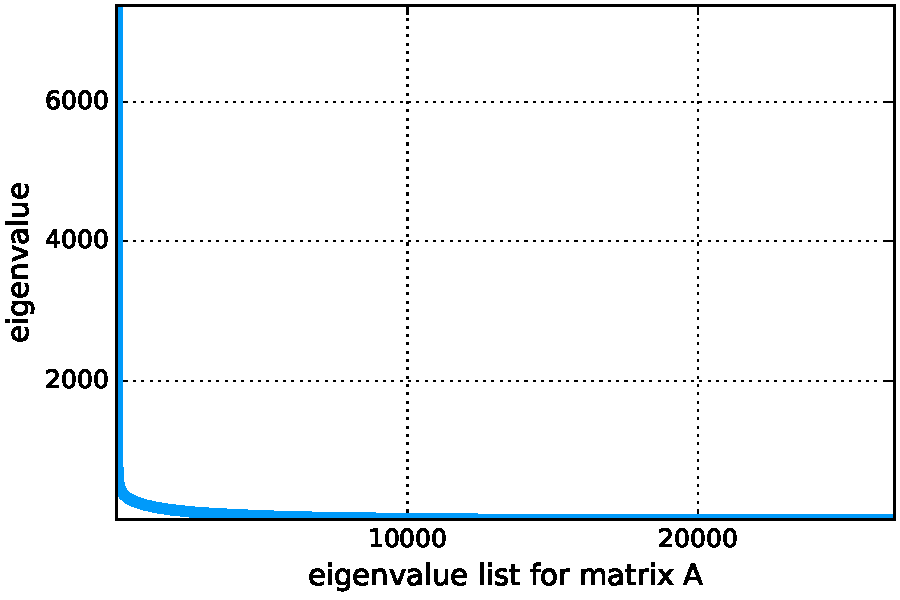
\includegraphics[width=0.48\textwidth]{fig/eigs.pdf}
    \hskip 0.2cm
	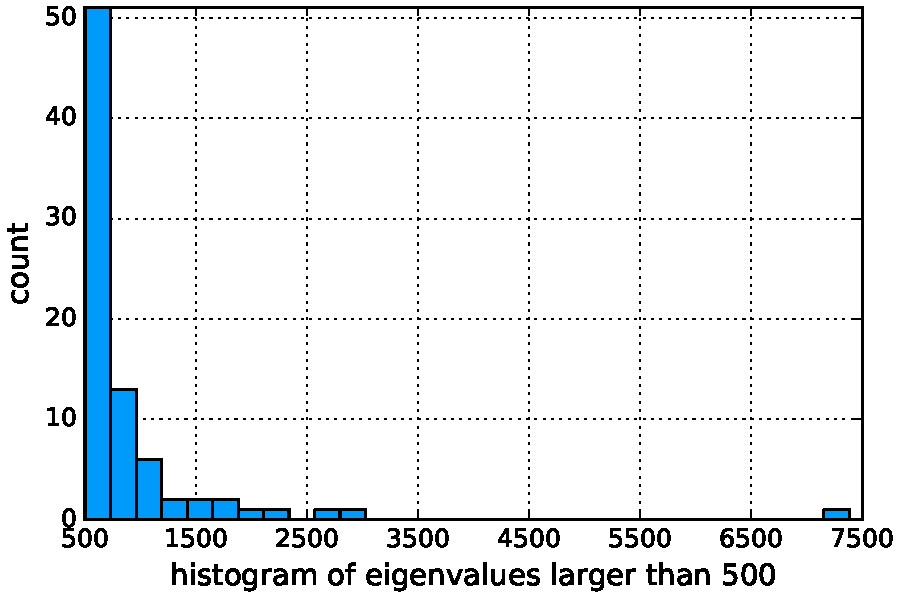
\includegraphics[width=0.48\textwidth]{fig/eig_large.pdf}
	\caption{\small
  		\textbf{Left}: Eigenvalues of matrix $A$.
          They are sorted for visualization.
          We can see a small portion of very large values.
        \textbf{Right}: Detailed distribution for large eigenvalues.}
	\label{fig:eig}
\end{figure}
